\documentclass[tikz]{standalone}
\usepackage{circuitikz}
\begin{document}


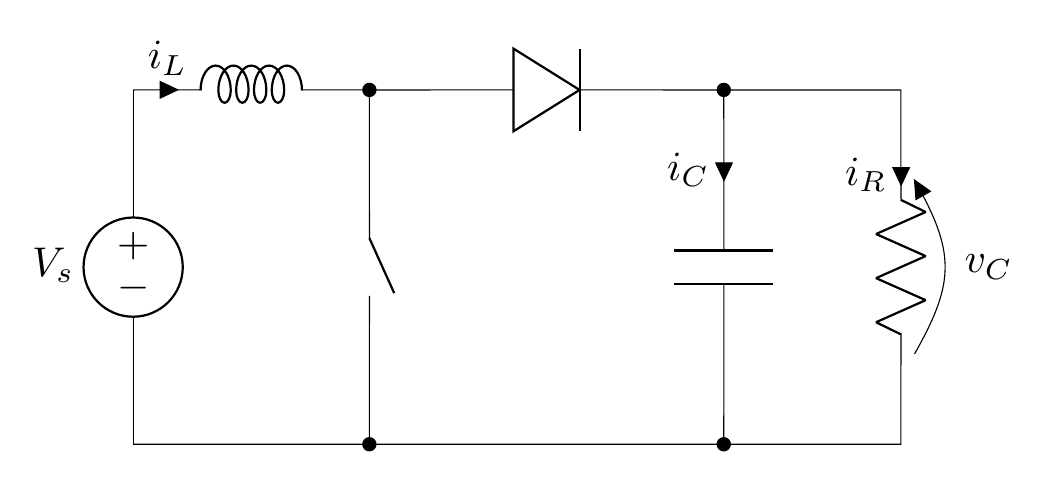
\begin{tikzpicture}[scale=1.5, transform shape]

\draw (0,3) to[american voltage source,l_=$V_s$] (0,0);
\tikzset{voltage dir=RP}
\draw (0,3) to [L,i>^=$i_L$]++(2,0) node[](A){} -- ++(0.5,0) to [D]  ++(2,0) -- ++(0.5,0) node[](B){} -| ++(1.5,-0.5) to [R,v^=$v_C$,i>_=$i_R$]++(0,-2) |- (0,0);
\draw (A.center)  to  [nos,*-*] ++(0,-3); 
\draw (B.center) to [C,i>_=$i_C$,*-*] ++(0,-3);

\end{tikzpicture}


\end{document}
